\documentclass{article}
\usepackage[margin=1in]{geometry}
\usepackage{amsmath}
\usepackage{amssymb}
\usepackage{amsthm}
\usepackage{bm}
\usepackage{hyperref}
\usepackage{graphicx}
\usepackage{caption}
\usepackage{listings}
\usepackage{xcolor}
\usepackage{float}
\usepackage{booktabs}
\usepackage{longtable}
\usepackage{multirow}
\usepackage{placeins}
\graphicspath{{figures/}}

% Code style
\lstdefinestyle{code}{
  basicstyle=\ttfamily\small,
  numbers=left,
  numberstyle=\tiny,
  numbersep=8pt,
  keywordstyle=\color{blue},
  commentstyle=\color{teal!70!black},
  stringstyle=\color{orange!70!black},
  showstringspaces=false,
  breaklines=true,
  frame=single,
  framerule=0.3pt,
  rulecolor=\color{black!15}
}
\lstset{style=code}

\title{Multimodal LLM Frontiers: Vision-Language, Audio-Video Fusion, and Alignment Adapters}
\author{}
\date{\today}

\begin{document}
\maketitle

\section{Text + Image: CLIP, BLIP, GPT-4V}
\subsection{Overview}
Vision-language models encode each modality separately before aligning them in a shared space, as shown in Figure~\ref{fig:multimodal_pipeline_en}. Text encoders (Transformers) ingest prompts, while image encoders (ViT, ConvNeXt) produce visual tokens; a fusion layer or adapter feeds the large language model decoder.
\begin{figure}[H]
  \centering
  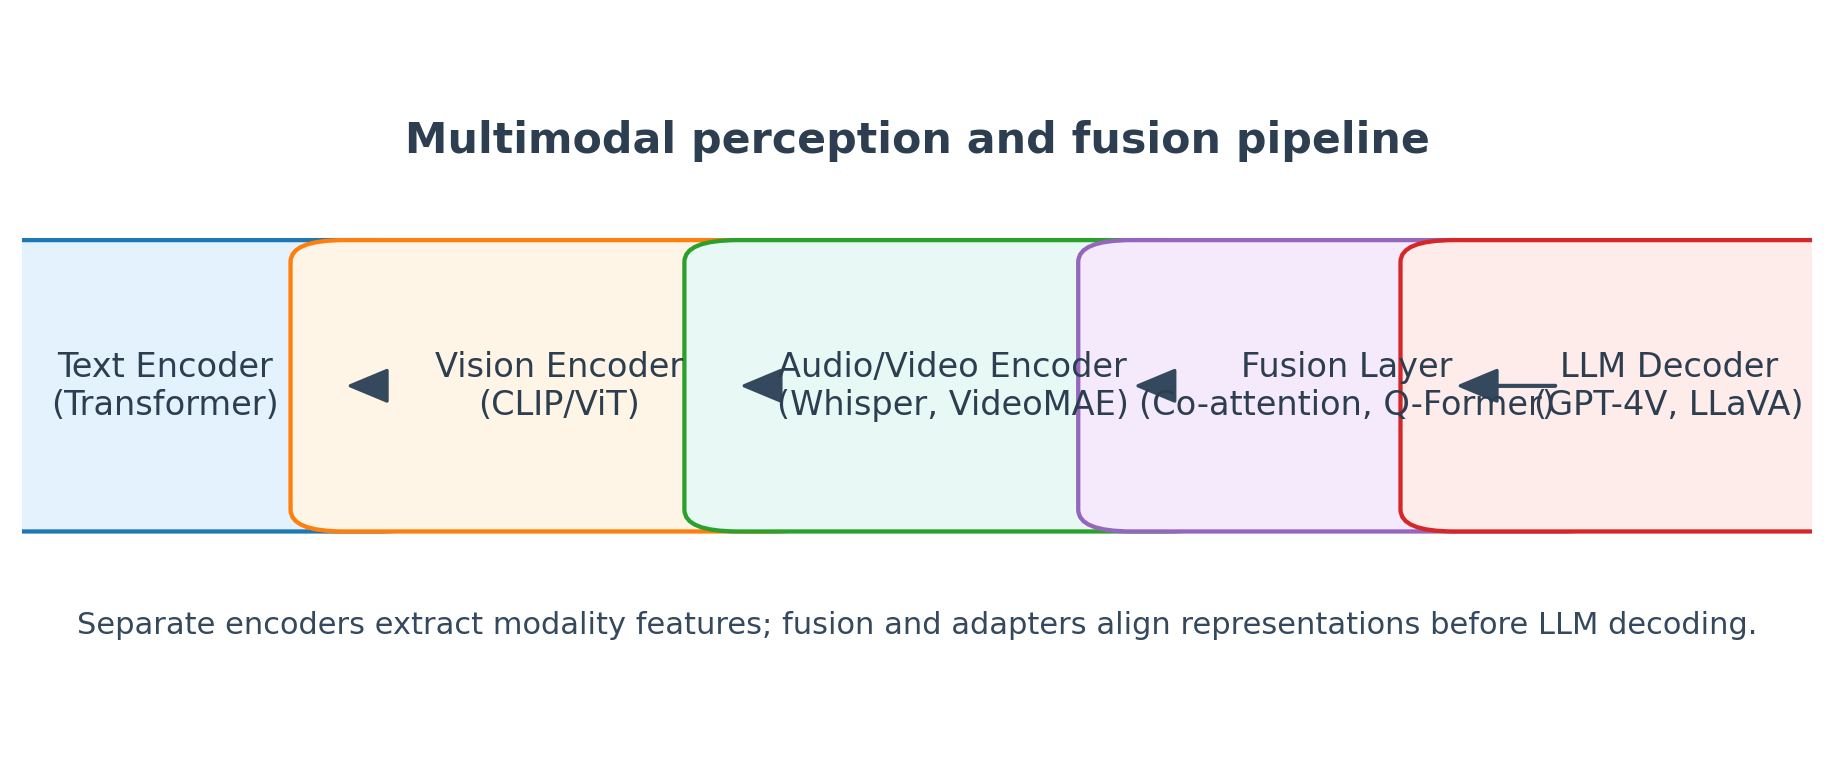
\includegraphics[width=0.95\textwidth]{multimodal_pipeline.png}
  \caption{Multimodal perception pipeline combining text, image, and audio encoders before fusion and LLM decoding.}
  \label{fig:multimodal_pipeline_en}
\end{figure}

\subsection{CLIP: Contrastive pre-training}
\begin{itemize}
  \item Paired text and image encoders output normalized embeddings.
  \item InfoNCE loss pushes matched pairs together and mismatched pairs apart across large web corpora.
  \item Enables zero-shot classification, cross-modal retrieval, and prompt-guided generative tasks.
\end{itemize}

\subsection{BLIP and BLIP-2: Generative alignment}
\begin{itemize}
  \item BLIP introduces a Vision Transformer plus Q-Former that maps visual features into query tokens consumed by a language decoder.
  \item BLIP-2 keeps the language model frozen (Flan-T5, OPT) and trains only the Q-Former bridge, drastically reducing compute.
  \item Supports captioning, VQA, dialogue grounding, and instruction tuning with generated image-text pairs.
\end{itemize}

\subsection{GPT-4V and open-source analogues}
\begin{itemize}
  \item GPT-4V accepts multimodal prompts, handling OCR, chart reasoning, spatial reasoning, and safety-guided refusal.
  \item LLaVA aligns CLIP ViT features with LLaMA embeddings via a simple projection and supervised instruction tuning.
  \item MiniGPT-4 leverages BLIP-2 Q-Former with Vicuna, using curated descriptive captions to bootstrap alignment.
\end{itemize}

\section{Text + Audio / Video / Sensor Fusion}
\subsection{Audio fusion}
\begin{itemize}
  \item Encoders: Whisper, wav2vec 2.0, HuBERT, or EnCodec for compressed representations.
  \item Tasks: speech recognition, speech translation, audio question answering, music captioning.
  \item Retrieval: contrastive objectives align text and audio vectors, powering query-to-sound or humming search.
\end{itemize}

\subsection{Video fusion}
\begin{itemize}
  \item Temporal encoders (VideoMAE, TimeSformer) tokenize frames and attend over space-time patches.
  \item Fusion strategies send summarized video features to language decoders through cross-attention modules.
  \item Applications: video captioning, video QA, highlight detection, autonomous driving perception.
  \item Long-form handling: keyframe extraction, hierarchical memory, and video-RAG to retrieve relevant segments.
\end{itemize}

\subsection{Sensor fusion}
\begin{itemize}
  \item Modalities include IMU (gyroscope, accelerometer), radar, LiDAR, temperature, biosignals.
  \item Feature engineering converts high-frequency signals into tokens via spectrograms, wavelets, or discretization.
  \item Use cases: robotics, industrial IoT anomaly detection, healthcare monitoring, smart buildings.
  \item Challenges: asynchronous sampling, noise, and limited labeled data; mitigated via self-supervised pretraining and domain adaptation.
\end{itemize}

\section{Alignment and Adapter Design}
\subsection{Adapter landscape}
Figure~\ref{fig:alignment_adapters_en} highlights projection heads, cross-modal adapters, and task heads that mediate heterogeneous representations.
\begin{figure}[H]
  \centering
  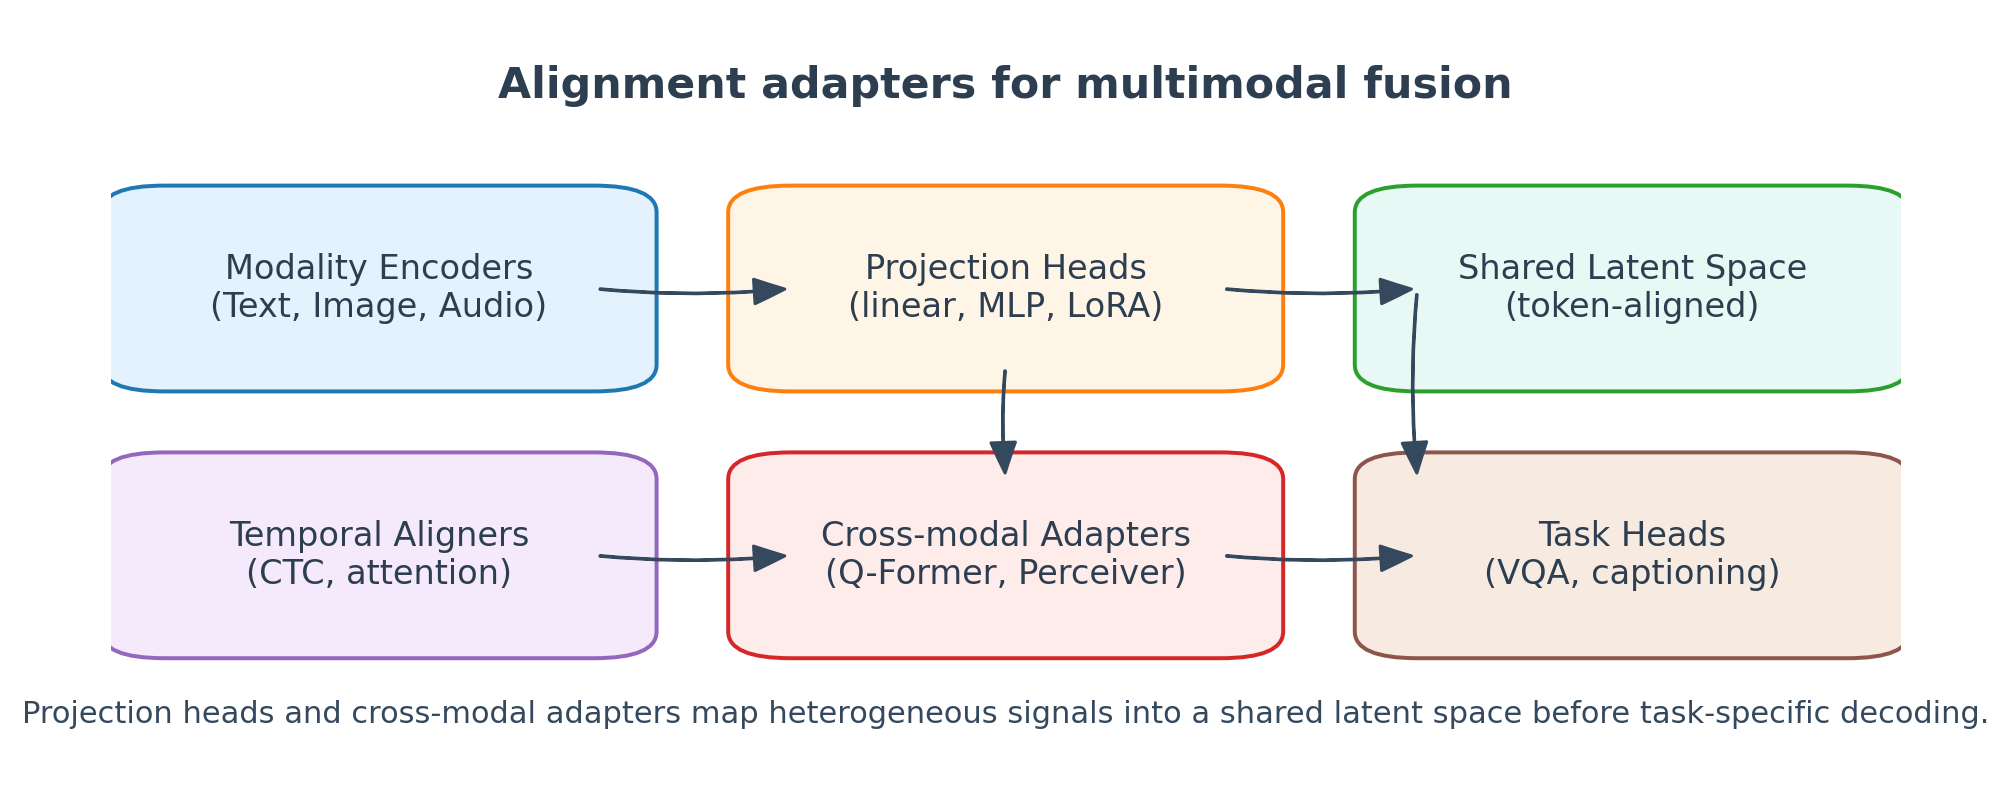
\includegraphics[width=0.95\textwidth]{alignment_adapters.png}
  \caption{Adapters that align modality encoders into shared latent spaces before task-specific heads.}
  \label{fig:alignment_adapters_en}
\end{figure}

\subsection{Projection layers}
\begin{itemize}
  \item Linear or MLP projections match dimensionality with minimal compute.
  \item LoRA and bottleneck adapters fine-tune frozen backbones with low-rank updates.
  \item Soft prompt tuning injects modality information as virtual tokens in the language model.
\end{itemize}

\subsection{Cross-modal adapters}
\begin{itemize}
  \item Q-Former distills visual features into fixed-length queries consumed by LLMs.
  \item Perceiver and PerceiverIO leverage cross-attention to handle arbitrary modalities and lengths.
  \item Token pruning and dynamic routing reduce redundancy for long video/audio streams.
\end{itemize}

\subsection{Training objectives}
\begin{itemize}
  \item Contrastive losses (InfoNCE, triplet) for retrieval alignment.
  \item Masked multimodal modeling (e.g., BEiT-3) to predict masked tokens across modalities.
  \item Instruction tuning with multimodal dialogues to teach reasoning grounded in visual/audio evidence.
  \item Multimodal RAG that retrieves image/audio snippets to augment language prompting.
\end{itemize}

\subsection{Case study: LLaVA fine-tuning}
\begin{enumerate}
  \item Extract CLIP ViT-L/14 features for images.
  \item Apply a linear projection into the LLaMA embedding space.
  \item Supervised fine-tune on ~150K multimodal instruction pairs.
  \item Evaluate on VQA, captioning, chart/question benchmarks; expand with self-instruct data generation.
\end{enumerate}

\section*{Operational recommendations}
\begin{itemize}
  \item Curate synchronized multimodal datasets; align timestamps and filter low-quality samples to prevent modality drift.
  \item Prefer modular adapters (LoRA, prompt tuning) to avoid full model retraining; enable rapid domain adaptation.
  \item Establish safety audits for hallucinations, bias, and misinformation—especially in sensitive visual/audio domains.
  \item Combine multimodal RAG and tool invocation for knowledge grounding, diagnostics, and real-world control loops.
\end{itemize}

\section*{Further reading}
\begin{itemize}
  \item Radford et al. ``Learning Transferable Visual Models from Natural Language Supervision.'' ICML, 2021.
  \item Li et al. ``BLIP-2: Bootstrapping Language-Image Pre-training with Frozen Image Encoders and Large Language Models.'' ICML, 2023.
  \item OpenAI. ``GPT-4V(ision) System Card.'' Technical Report, 2023.
  \item Alayrac et al. ``Flamingo: a Visual Language Model for Few-Shot Learning.'' NeurIPS, 2022.
  \item Bai et al. ``Q-Former: Querying Transformer for Multi-modal Interaction.'' arXiv, 2023.
\end{itemize}

\end{document}

